%%%%%%%%%%%%%%%%%%%%%%%%%%%%%%%%%%%%%%%%%
% Wenneker Article
% LaTeX Template
% Version 2.0 (28/2/17)
%
% This template was downloaded from:
% http://www.LaTeXTemplates.com
%
% Authors:
% Vel (vel@LaTeXTemplates.com)
% Frits Wenneker
%
% License:
% CC BY-NC-SA 3.0 (http://creativecommons.org/licenses/by-nc-sa/3.0/)
%
%%%%%%%%%%%%%%%%%%%%%%%%%%%%%%%%%%%%%%%%%

%----------------------------------------------------------------------------------------
%	PACKAGES AND OTHER DOCUMENT CONFIGURATIONS
%----------------------------------------------------------------------------------------

\documentclass[10pt, a4paper, twocolumn]{article} % 10pt font size (11 and 12 also possible), A4 paper (letterpaper for US letter) and two column layout (remove for one column)

%%%%%%%%%%%%%%%%%%%%%%%%%%%%%%%%%%%%%%%%%
% Wenneker Article
% Structure Specification File
% Version 1.0 (28/2/17)
%
% This file originates from:
% http://www.LaTeXTemplates.com
%
% Authors:
% Frits Wenneker
% Vel (vel@LaTeXTemplates.com)
%
% License:
% CC BY-NC-SA 3.0 (http://creativecommons.org/licenses/by-nc-sa/3.0/)
%
%%%%%%%%%%%%%%%%%%%%%%%%%%%%%%%%%%%%%%%%%

%----------------------------------------------------------------------------------------
%	PACKAGES AND OTHER DOCUMENT CONFIGURATIONS
%----------------------------------------------------------------------------------------

\usepackage[english]{babel} % English language hyphenation

\usepackage{microtype} % Better typography

\usepackage{amsmath,amsfonts,amsthm} % Math packages for equations

\usepackage[svgnames]{xcolor} % Enabling colors by their 'svgnames'

\usepackage[hang, small, labelfont=bf, up, textfont=it]{caption} % Custom captions under/above tables and figures

\usepackage{booktabs} % Horizontal rules in tables

\usepackage{lastpage} % Used to determine the number of pages in the document (for "Page X of Total")

\usepackage{graphicx} % Required for adding images

\usepackage{enumitem} % Required for customising lists
\setlist{noitemsep} % Remove spacing between bullet/numbered list elements

\usepackage{sectsty} % Enables custom section titles
\allsectionsfont{\usefont{OT1}{phv}{b}{n}} % Change the font of all section commands (Helvetica)

%----------------------------------------------------------------------------------------
%	MARGINS AND SPACING
%----------------------------------------------------------------------------------------

\usepackage{geometry} % Required for adjusting page dimensions

\geometry{
	top=1cm, % Top margin
	bottom=1.5cm, % Bottom margin
	left=2cm, % Left margin
	right=2cm, % Right margin
	includehead, % Include space for a header
	includefoot, % Include space for a footer
	%showframe, % Uncomment to show how the type block is set on the page
}

\setlength{\columnsep}{7mm} % Column separation width

%----------------------------------------------------------------------------------------
%	FONTS
%----------------------------------------------------------------------------------------

\usepackage[T1]{fontenc} % Output font encoding for international characters
\usepackage[utf8]{inputenc} % Required for inputting international characters

\usepackage{XCharter} % Use the XCharter font

%----------------------------------------------------------------------------------------
%	HEADERS AND FOOTERS
%----------------------------------------------------------------------------------------

\usepackage{fancyhdr} % Needed to define custom headers/footers
\pagestyle{fancy} % Enables the custom headers/footers

\renewcommand{\headrulewidth}{0.0pt} % No header rule
\renewcommand{\footrulewidth}{0.4pt} % Thin footer rule

\renewcommand{\sectionmark}[1]{\markboth{#1}{}} % Removes the section number from the header when \leftmark is used

%\nouppercase\leftmark % Add this to one of the lines below if you want a section title in the header/footer

% Headers
\lhead{} % Left header
\chead{\textit{\thetitle}} % Center header - currently printing the article title
\rhead{} % Right header

% Footers
\lfoot{} % Left footer
\cfoot{} % Center footer
\rfoot{\footnotesize Page \thepage\ of \pageref{LastPage}} % Right footer, "Page 1 of 2"

\fancypagestyle{firstpage}{ % Page style for the first page with the title
	\fancyhf{}
	\renewcommand{\footrulewidth}{0pt} % Suppress footer rule
}

%----------------------------------------------------------------------------------------
%	TITLE SECTION
%----------------------------------------------------------------------------------------

\newcommand{\authorstyle}[1]{{\large\usefont{OT1}{phv}{b}{n}\color{DarkRed}#1}} % Authors style (Helvetica)

\newcommand{\institution}[1]{{\footnotesize\usefont{OT1}{phv}{m}{sl}\color{Black}#1}} % Institutions style (Helvetica)

\usepackage{titling} % Allows custom title configuration

\newcommand{\HorRule}{\color{DarkGoldenrod}\rule{\linewidth}{1pt}} % Defines the gold horizontal rule around the title

\pretitle{
	\vspace{-30pt} % Move the entire title section up
	\HorRule\vspace{10pt} % Horizontal rule before the title
	\fontsize{32}{36}\usefont{OT1}{phv}{b}{n}\selectfont % Helvetica
	\color{DarkRed} % Text colour for the title and author(s)
}

\posttitle{\par\vskip 15pt} % Whitespace under the title

\preauthor{} % Anything that will appear before \author is printed

\postauthor{ % Anything that will appear after \author is printed
	\vspace{10pt} % Space before the rule
	\par\HorRule % Horizontal rule after the title
	\vspace{20pt} % Space after the title section
}

%----------------------------------------------------------------------------------------
%	ABSTRACT
%----------------------------------------------------------------------------------------

\usepackage{lettrine} % Package to accentuate the first letter of the text (lettrine)
\usepackage{fix-cm}	% Fixes the height of the lettrine

\newcommand{\initial}[1]{ % Defines the command and style for the lettrine
	\lettrine[lines=3,findent=4pt,nindent=0pt]{% Lettrine takes up 3 lines, the text to the right of it is indented 4pt and further indenting of lines 2+ is stopped
		\color{DarkGoldenrod}% Lettrine colour
		{#1}% The letter
	}{}%
}

\usepackage{xstring} % Required for string manipulation

\newcommand{\lettrineabstract}[1]{
	\StrLeft{#1}{1}[\firstletter] % Capture the first letter of the abstract for the lettrine
	\initial{\firstletter}\textbf{\StrGobbleLeft{#1}{1}} % Print the abstract with the first letter as a lettrine and the rest in bold
}

%----------------------------------------------------------------------------------------
%	BIBLIOGRAPHY
%----------------------------------------------------------------------------------------

\usepackage[backend=bibtex,style=authoryear,natbib=true]{biblatex} % Use the bibtex backend with the authoryear citation style (which resembles APA)

\addbibresource{example.bib} % The filename of the bibliography

\usepackage[autostyle=true]{csquotes} % Required to generate language-dependent quotes in the bibliography
 % Specifies the document structure and loads requires packages

%----------------------------------------------------------------------------------------
%	ARTICLE INFORMATION
%----------------------------------------------------------------------------------------

\title{Central Operativa SAL/T} % The article title

\author{
	\authorstyle{Matías Sambrizzi \textsuperscript{1} and Fernando Iglesias\textsuperscript{1}} % Authors
	\newline\newline % Space before institutions
	\textsuperscript{1}\institution{Universidad de Buenos Aires, Buenos Aires, Argentina}\\ % Institution 1
}

% Example of a one line author/institution relationship
%\author{\newauthor{John Marston} \newinstitution{Universidad Nacional Autónoma de México, Mexico City, Mexico}}

% \date{\today} % Add a date here if you would like one to appear underneath the title block, use \today for the current date, leave empty for no date

%----------------------------------------------------------------------------------------

\begin{document}

\maketitle % Print the title

\thispagestyle{firstpage} % Apply the page style for the first page (no headers and footers)

%----------------------------------------------------------------------------------------
%	ABSTRACT
%----------------------------------------------------------------------------------------

\textit{\textbf{Resumen-}}   En el presente artículo se presentan los avances del desarrollo de una arquitectura modular para la Central Operativa \textit{SAL/T} basado en el paradigma de Internet de las Cosas (IoT). Este proyecto es el complemento en materia de \textit{software} de un prototipo realizado para Trenes Argentinos, entidad que se ocupa de gestionar y operar la red ferroviaria de la Argentina.
\newline

\textit{\textbf{Keywords-}}  MQTT, JSON, ...


%----------------------------------------------------------------------------------------
%	ARTICLE CONTENTS
%----------------------------------------------------------------------------------------

\section{Motivación y Contexto}

Las formaciones ferroviarias cuentan con diferentes sistemas de seguridad a bordo, siendo estos, equipos que se encargan de supervisar el correcto funcionamiento de los subsistemas críticos. Ante una falla en uno de los subsistemas, una formación ferroviaria se detiene inmediatamente por la activación automática de las señales de corte de tracción (\textit{CT}) y frenado de emergencia (\textit{FE}). En esta situación, el conductor debe llevar la formación a un lugar seguro para que los pasajeros puedan descender y, posteriormente, trasladarla a un taller para que pueda ser reparada.

El \textit{SAL/T} \footnote{referencia al artículo de Di Vito}, según sus siglas, Sistema de Aislamiento Limitado o Total, es un sistema que le permite al maquinista de una formación ferroviaria la posibilidad de activar y desactivar del modo aislado limitado. En este modo, el equipo permite la circulación de la formación al desactivar las señales de corte de tracción y freno de emergencia generadas por los otros subsistemas. Para que esta operación se realice de forma segura, se debe monitorear la velocidad de la formación tal que sea posible evitar que supere cierto valor máximo. 

A partir del prototipo físico del SAL/T previamente mencionado, se presentan los avances en el desarrollo de una central operativa, es una plataforma web que cuenta con una unidad lógica de compartición y empaquetado de software, que posibilita la administación, la configuración y el monitoreo en tiempo real de la información recibida y transmitida por parte de cada dispositivo SAL/T.

\section{Descripción de la problemática a resolver}

Los subsistemas asociados al SAL/T como la seguridad de puertas, el sistema de hombre vivo y la protección de coche a la deriva; son críticos debido a que, en caso de fallar, pueden ocasionar lesiones o muertes de personas, dañar el medio ambiento e incluso generar pérdidas materiales. 

En efecto, la central operativa permite la administación y configuración de forma remota los dispositivos de supervisión de seguridad de cada formación ferroviaria, la visualización de los diferentes parámetros de interés involucrados tal que se encuentre al alcance de una o más personas asignadas dentro de una entidad y de este modo, sea posible optimizar la toma de decisiones.

Como consecuencia de lo expresado previamente, se ha realizado el diseño de una arquitectura versátil y confiable en términos de capacidad de procesamiento y de almacenamiento de la información.

En la sección III, según el \textit{stack} de una solución IoT, se presentan cada una de las tecnologías utilizadas. Luego, en la sección IV se exponen las conclusiones y por último, en la sección V, se presentan los próximos pasos del trabajo.


\section{Arquitectura propuesta}

En el marco del presente trabajo, la arquitectura esta estratificada en capas
tal como se ilustra en la fiugra X. A continuación se describen cada una de ellas

\begin{figure}[ht]
\centering 
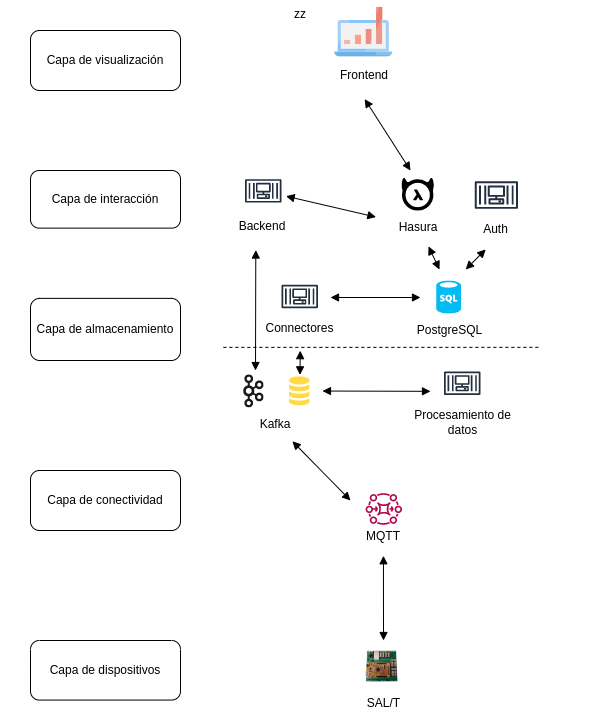
\includegraphics[width=.5\textwidth]{diagram.png}
\caption{Arquitectura de la Central Operativa SAL/T.}
\label{fig:diagBloques}
\end{figure}

\subsection{Capa de dispositivos}

Sobre la base de un prototipo del Sistema de Aislamiento Limitado o Total, se propuso la migración al kit de desarrolo \textit{Nucleo F429} dado que cuenta con un mayor soporte y funcionalidades de seguridad. Actualmente, se está desarrollando un cliente \textit{MQTT}que permite la publicación de la información proveniente de los subsistemas de falla, la velocidad de la información, entre otras variables; y llegado el caso, el dispositivo pueda realizar la lectura de diferentes parámetros configurables, como por ejemplo, los perfiles de \textit{chopeo} que un operario publique desde la Central Operativa SAL/T para una formación ferroviaria.  


\subsection{Capa de conectividad}

Para la comunicación entre los dispositivos \textit{SAL/T} y la capa de almacenamiento, se utiliza un \textit{Broker MQTT} que oficia de orquestador entre el cliente, dispositivo \textit{SAL/T}, que publica los mensajes y aquel que se suscribe, el sistema \textit{Kafka}, para la lectura de la información y su posterior procesamiento. 

Dado que los mensajes intercambiados entre las partes contienen información sensible, se ha optado por agregar la capa de seguridad \textit{TLS}. En este sentido, resulta indispensable utilizar el certificado \textit{X509} para prevenir ataques del tipo \textit{adversary-in-the-middle} y utilizar certificados emitidos por autoridades reconocidas.


\subsection{Capa de almacenamiento}

La capa de almacenamiento por un lado se encuentra constituida por el sistema distribuido \textit{Kafka} que se encarga
de almacenar los datos de la aplicación. Entre ellos se destacan los mensajes MQTT enviados
por los dispositivos SAL/T, como también la información referida a las formaciones y a los SAL/T que las ocupan. 
Ademas, se tienen servicios de procesamiento de datos que se encargan de adaptar la información de los tópicos en
datos que posteriormente serán consumidos por los servicios que integran la capa superior. Por otro lado,
se tiene una base de datos SQL que se utiliza para almacenar los datos del servicio de autenticación y 
Hasura. Los conectores se encargan de insertar los datos que se quieran disponer a la capa de 
visualización.

\subsection{Capa de interacción}

La capa de interacción se encuentra conformada por tres unidades. Por un lado, se ha desarrollado en el lenguaje \textit{Kotlin} en conjunto con el \textit{framework} \textit{Ktor} un microservicio de autenticación donde es posible la gestión de los usuarios con sus respectivos roles y también el \textit{backend}. Entre sus tareas principales se encuentran las relacionadas al protocolo \textit{MQTT} para la actualización de los certificados que brindan seguridad a las comunicaciones, mediante el uso de la capa de seguridad \textit{TLS}, y la indexación de los eventos que se publiquen en tiempo real; como la configuración general que permite el funcionamiento integral de los servicios y módulos dispuestos en el sistema.

Además, se dispone del motor \textit{Hasura}, el cual se encuentra conectado a una base de datos relacional (\textit{PostgreSQL}) basado en el lenguaje de consulta estructurado \textit{SQL}, que permite exponer una \textit{API GraphQL} a aquellos clientes que deseen obtener una visualización del modelo de datos propuesto en que se conjuga la información de cada formación ferroviar con su correspondiente dispositivo \textit{SAL/T} y diseño destinado al \textit{frontend}. Más aún, el enlace permite realizar modificaciones y hasta remociones de las columnas propuestas en el modelo.


\subsection{Capa de visualizacion}

En la capa de visualización se desarrollo una aplicación web utilizando el lenguaje
de programación Typescript y el framework React.

En esta capa, se ha utilizato el lenguaje de programación \textit{TypeScript} junto con la biblioteca gráfica \textit{React} para brindar una web reactiva en el que se elaboraron los formularios, las tablas y los paneles a partir de la explotación en de los datos almacenados en la base de datos. Cabe destacar que la plataforma web se encuentra condicionada por el rol y la entidad a la que pertenece cada usuario.  


\section{Conclusiones}

En este trabajo se presentan las principales características del diseño de una arquitectura en materia de \textit{software} y de \textit{firmware} para la operabilidad de los dispositivos SAL/T.

Entre los módulos desarrollados, se posibilita la visualización de los usuarios y los dispositivos de cada entidad ofreciendo una solución sencilla y escalable. También, se cuenta la ingestión de la información recibida desde los dispositivos permitiendo una alta disponibilidad y operabilidad de los recursos. Por último, se cuenta con un microservicio destinado a la gestión de usuarios y perfiles que posee una alta tolerancia a fallos y adaptable.


\section{Próximos pasos}

En la actualidad, se encuentra en desarrollo propiciar al operario enviar comandos de control a los dispositivos activos que tenga asignados, brindar la connfiguración de los parámetros de cada dispositivo y de ser deseable su correspondiente modificación y finalmente, brindar la seguridad en las comunicaciones agregando la capa \textit{TLS} en el protocolo \textit{MQTT}. 


%----------------------------------------------------------------------------------------
%	BIBLIOGRAPHY
%----------------------------------------------------------------------------------------

\printbibliography[title={Bibliography}] % Print the bibliography, section title in curly brackets

%----------------------------------------------------------------------------------------

\end{document}
